\chapter{Implementation strategies}

Due to the structural differences of SPN- and Feistel network-based ciphers, we
shall analyze these two separately.

\section{Strategies for SPN}

Three implementation strategies for substitution-permutation networks are
introduced by \cite{implx86:2014}:

\begin{itemize}
    \item Table-based implementations
    \item \texttt{vperm} implementations
    \item Bitslice implementations
\end{itemize}

\subsection{Table-based}

Table-driven programming is a simple way to increase performance of operations
by tabulating the results, therefore requiring only a single memory access to
acquire the result. This approach is obviously limited to manageable table
sizes, so while tabulating a function like the AES S-box
$S_{AES}:\F{8}\rightarrow \F{8}$ requires only $2^{11}$ space,
tabulating the \texttt{GIFT} permutation layer
$P_{GIFT}:\F{64}\rightarrow \F{64}$ would require
$2^{70}$ space, which is totally unfeasible.

A common approach is to tabulate the output of each S-box, including the
diffusion layer, and then XORing the results together. Let $n$ denote the
internal cipher state size and $s$ the size of a single S-box in bits. For each
S-box $S_i,i\in\{0,\dots,\frac{n}{s}\}$, we can construct a mapping
$T_i:\F{s}\rightarrow \F{n}$ representing substitution with subsequent
permutation of that single S-box. The cipher state before round key addition is
then given by $\bigoplus_{i=0}^{\frac{n}{s}-1}{T_i(m_i)}$ for each $s$-bit
message chunk $m_i$. This approach requires space of
$\frac{n}{s}|\F{s}|n=\frac{n^2 2^s}{s}$ bits, which, for \texttt{GIFT-64},
results in a manageable size of $\frac{64^2 2^4}{4}=2^{14}$ bits which equals
$16$ KiB.

\subsubsection{Constructing the tables}

For \texttt{GIFT-64}, table construction is relatively straightforward and can
be done as follows:

\begin{lstlisting}[caption={Table construction algorithm}, label={lst:tables}, escapechar=|]
    tables <- [][]
    for sbox_index from 0 to 15 do
        for sbox_input from 0 to 15 do|\label{lst:tablesbox}|
            output <- sbox(sbox_input)
            output <- permute(output << (4 * sbox_index))
            tables[sbox_index][sbox_input] <- output
\end{lstlisting}

Implementing this algorithm gives us the following table representing the first
and second S-box.

\[
    \begin{array}{l|l|l|c}
        x & T_0(x) & T_1(x) & \dots \\
        \hline
        0x0 & 0x1               & 0x1000000000000   & \dots \\
        0x1 & 0x8000000020000   & 0x800000002       & \dots \\
        0x2 & 0x400000000       & 0x40000           & \dots \\
        0x3 & 0x8000400000000   & 0x800040000       & \dots \\
        0x4 & 0x400020000       & 0x40002           & \dots \\
        0x5 & 0x8000400020001   & 0x1000800040002   & \dots \\
        0x6 & 0x20001           & 0x1000000000002   & \dots \\
        0x7 & 0x8000000000001   & 0x1000800000000   & \dots \\
        0x8 & 0x20000           & 0x2               & \dots \\
        0x9 & 0x8000400000001   & 0x1000800040000   & \dots \\
        0xa & 0x8000000020001   & 0x1000800000002   & \dots \\
        0xb & 0x400020001       & 0x1000000040002   & \dots \\
        0xc & 0x400000001       & 0x1000000040000   & \dots \\
        0xd & 0x0               & 0x0               & \dots \\
        0xe & 0x8000000000000   & 0x800000000       & \dots \\
        0xf & 0x8000400020000   & 0x800040002       & \dots
    \end{array}
\]

The tables for \texttt{GIFT-128} can be generated in a similar way by looping
through all 32 S-boxes instead of 16 on line \ref{lst:tablesbox}.

\subsection{Using \texttt{vperm}}

Nowadays, most instructions set architectures support single-instruction,
multiple-data processing. The idea of such an SIMD system is to work on
multiple data stored in vectors at once to speed up calculations. For A64, two
types of vector processing are available:

\begin{enumerate}
    \item Advanced SIMD, known as NEON
    \item Scalable Vector Extension (SVE)
\end{enumerate}

We will take a look at NEON as this is the type of vector processing supported
by the Cortex-A73 processor.

\subsubsection{ARM Neon}

The register file of the NEON unit is made up of 32 quad-word (128-bit)
registers \texttt{V[0-31]}, each extending the standard 64-bit floating-point
registers \mbox{\texttt{D[0-31]}}. These registers are divided into equally
sized lanes on which the vector instructions operate. Valid ways to interpret
for example the register \texttt{V0} are:

\begin{figure}[h!]
    \centering
    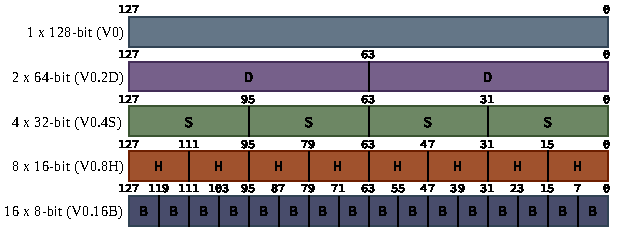
\includegraphics[width=\textwidth]{Figures/V_register.pdf}
    \caption{Divisions of the V0 register}
\end{figure}

NEON instructions interpret their operands' layouts (i.e. lane count and width)
through the use of suffixes such as \texttt{.4S} or \texttt{.8H}. For example,
adding eight 16-bit halfwords from register \texttt{V1} and \texttt{V2}
together and storing the result in \texttt{V0} can be done as follows:

\begin{center}
    \texttt{ADD V0.8H, V1.8H, V2.8H}
\end{center}

\begin{figure}[h!]
    \centering
    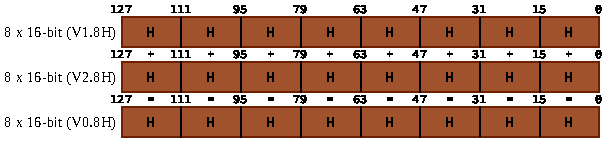
\includegraphics[width=\textwidth]{Figures/vector_add.pdf}
    \caption{Addition of two vector registers}
\end{figure}

The plenitude of different processing instructions allow flexible ways to
further speed up algorithms having reached their optimizational limit on
non-SIMD platforms. \texttt{vperm}, a general term standing for \textit{vector
permute}, is a common instruction on SIMD machines. Called \texttt{TBL} on
NEON, it is used for parallel table lookups and arbitrary permutations. It takes
two inputs to perform a lanewise lookup:

\begin{enumerate}
    \item A register with lookup values
    \item Two or more registers containing data
\end{enumerate}

\subsubsection{S-box lookup}

This instruction can be used to implement S-box lookup of all 16 S-boxes in a
single instruction. We do this by packing our 64-bit cipher state
$s=s_{15}||s_{14}||\dots||s_0$ into a vector register $V_0$. Because we can
only operate on whole bytes, we put each 4-bit S-box into an 8-bit lane which
neatly fits into the 128-bit registers. We then put the S-box itself into
register $V_1$ which will be used as the data register for the table lookup.

The confusion layer can now be performed through one \texttt{TBL} instruction:

\begin{center}
    \texttt{TBL V0.16B, V1.16B, V0.16B}
\end{center}

\begin{figure}[h!]
    \centering
    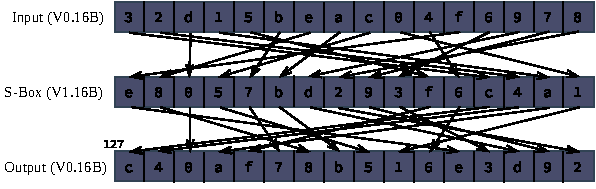
\includegraphics[width=\textwidth]{Figures/tbl_example.pdf}
    \caption{Performing the S-Box lookup in parallel}
\end{figure}

\subsection{Bitslicing}

Bitslicing refers to the technique of splitting up $n$ bits into $m$ slices to
achieve a more efficient representation to operate on. The structure of
\texttt{GIFT} naturally offers possibilities for bitslicing. We split the
cipher state bits $b_{63}b_{62}\dots b_0$ into four slices $S_i,
i\in\{0,1,2,3\}$ such that the $i$-th slice contains all $i$-th bits of the
individual S-boxes. This is equivalent to transposing the bit matrix.

\[
    S=\begin{bmatrix}
        S_0\\
        S_1\\
        S_2\\
        S_3
    \end{bmatrix}
    =\begin{bmatrix}
        b_{60}b_{56}b_{52}\dots b_0\\
        b_{61}b_{57}b_{53}\dots b_1\\
        b_{62}b_{58}b_{54}\dots b_2\\
        b_{63}b_{59}b_{55}\dots b_3
    \end{bmatrix}
\]

\subsubsection{Parallel S-Boxes}

This representation offers multiple advantages. We first note that computation
of the S-box can be executed in parallel, similar to the \texttt{vperm}
technique above. This can be done by finding an algorithmic way to apply the
S-box which has already been proposed by the original \texttt{GIFT} authors:

\begin{align*}
    S_1&\leftarrow S_1\oplus (S_0\land S_2) \\
    t&\leftarrow S_0\oplus (S_1\land S_3) \\
    S_2&\leftarrow S_2\oplus (t\lor S_1) \\
    S_0&\leftarrow S_3\oplus S_2 \\
    S_1&\leftarrow S_1\oplus S_0 \\
    S_0&\leftarrow \lnot S_0 \\
    S_2&\leftarrow S_2\oplus (t\land S_1) \\
    S_3&\leftarrow t
\end{align*}

This is very efficient as it only requires six XOR-, three AND and one OR
operation.

An important property of the permutation is the fact that bits always stay in
their slice. This means we can decompose the permutation $P$ into four
permutations $P_i,i\in\{0,1,2,3\}$ and apply these permutations
separately to each slice. One possible way to implement a permutation $P_i$ in
software is to mask off all bits individually, shift them to their correct
position and OR them together:

\[
    P_i(S_i)=\bigvee_{k=0}^{15}{(S_i\land m_i) \ll s_i}
\]

This approach requires $47$ operations, meaning all four permutations require
over $150$ operations which would present a major bottleneck to the round
function. We can improve on this by working on multiple message blocks at once
and using the aforementioned \texttt{vperm} instruction to implement the bit
shuffling. We then need only four instructions for the complete diffusion
layer.

\subsubsection{Using \texttt{vperm} for slice permutation}

We cannot use the \texttt{TBL} instruction directly as we need to shuffle
individual bits, but the smallest data we can operate on are bytes. We
therefore encrypt $8n$ messages at once which allows us to create bytewise
groupings. These messages are put into $4m$ registers with register $R_{4i}$
containing $S_0$, register $R_{4i+1}$ containing $S_1$ and so forth. With block
size $BS$ and register size $RS$, the following must hold:

\[
    8n\cdot BS=4m\cdot RS
\]

In the case of \texttt{GIFT-64} with $BS=64$ and ARM NEON with $RS=128$, we get

\[
    8n\cdot 64=4m\cdot 128\Leftrightarrow n=m
\]

$n=m=1$ would be a valid choice which yields eight messages divided into four
registers. We choose $n=m=2$ so we can directly utilize the algorithm for bit
packing presented by the original GIFT authors, although it is simple to adapt
this algorithm to only four registers and eight messages by adjusting the
\texttt{SWAPMOVE} shift and mask values.

\subsubsection{Packing the data into bitslice format}

Let $a,b,\dots,p$ be sixteen messages of length $64$ with subscripts denoting
individual bits. We first put these messages into eight SIMD registers
$V_0,V_1,\dots,V_7$:

\begin{alignat*}{3}
    V_0&=b||a\qquad V_4&&=j||&&i \\
    V_1&=d||c\qquad V_5&&=l||&&k \\
    V_2&=f||e\qquad V_6&&=n||&&m \\
    V_3&=h||g\qquad V_7&&=p||&&o
\end{alignat*}

We then use the \texttt{SWAPMOVE} technique to bring the data into bitslice
format. This operation operates on two registers $A,B$ using mask $M$ and shift
value $N$. It swaps bits in $A$ masked by $(M\ll N)$ with bits in $B$ masked by
$M$ in using only three XOR-, one AND- and two shift operations.

\begin{align*}
    &\text{SWAPMOVE}(A,B,M,N): \\
    &\qquad T=((A\gg N)\oplus B)\land M \\
    &\qquad B=B\oplus T \\
    &\qquad A=A\oplus (T\ll N) \\
\end{align*}

One caveat of this approach is the fact that NEON registers cannot be shifted
in their entirety due to the fact bits are not able to cross lanes. This leads
to the problem of being able to shift at most two lanes of 64 bits at once. We
thus need to implement the \texttt{shr(V,n)} and \texttt{shl(V,n)} operations
on our own. This can be done by first extracting the 64-bit lanes $a,b$ out of
$V=b||a$, shifting the lanes individually and finally shifting and ORing the
crossing bits back into the other lane.

\begin{alignat*}{2}
    &\text{shl}(V,n): \\
    &\qquad a,b&&=V[0],V[1] \\
    &\qquad c&&=(a\gg (64-n)) \\
    &\qquad a&&=(a\ll n) \\
    &\qquad b&&=(b\ll n)\lor c \\
    &\qquad V[0],V[1]&&=a,b
\end{alignat*}

The following operations group all $i$th bits of the messages $a,c,\dots,o$
into bytes and puts these into the lower half of the registers $V_{i\bmod 8}$.
The same is done for messages $b,d,\dots,p$, only differing in that the bytes
are put into the upper half of the registers.

\begin{align*}
    &\text{SWAPMOVE}(V_0,V_1,0x5555\dots 55,1) &\text{SWAPMOVE}(V_4,V_5,0x5555\dots 55,1) \\
    &\text{SWAPMOVE}(V_2,V_3,0x5555\dots 55,1) &\text{SWAPMOVE}(V_6,V_7,0x5555\dots 55,1) \\
    &\text{SWAPMOVE}(V_0,V_2,0x3333\dots 33,2) &\text{SWAPMOVE}(V_4,V_6,0x3333\dots 33,2) \\
    &\text{SWAPMOVE}(V_1,V_3,0x3333\dots 33,2) &\text{SWAPMOVE}(V_5,V_7,0x3333\dots 33,2) \\
    &\text{SWAPMOVE}(V_0,V_4,0x0f0f\dots 0f,4) &\text{SWAPMOVE}(V_1,V_5,0x0f0f\dots 0f,4) \\
    &\text{SWAPMOVE}(V_2,V_6,0x0f0f\dots 0f,4) &\text{SWAPMOVE}(V_3,V_7,0x0f0f\dots 0f,4) \\
\end{align*}

With $Ax=o_xm_xk_xj_xg_xe_xc_xa_x$ and $Bx=p_xn_xl_xi_xh_xf_xd_xb_x$ denoting
byte groups, our data now has the following permutation-friendly format:

\[
    \scriptsize
    \begin{array}{c|llllllll|llllllll}
        n & 15 & 14 & 13 & 12 & 11 & 10 & 9 & 8 & 7 & 6 & 5 & 4 & 3 & 2 & 1 & 0 \\
        \hline
        V_0 & B56 & B48 & B40 & B32 & B24 & B16 & B8  & B0 & A56 & A48 & A40 & A32 & A24 & A16 & A8  & A0 \\
        V_1 & B57 & B49 & B41 & B33 & B25 & B17 & B9  & B1 & A57 & A49 & A41 & A33 & A25 & A17 & A9  & A1 \\
        V_2 & B58 & B50 & B42 & B34 & B26 & B18 & B10 & B2 & A58 & A50 & A42 & A34 & A26 & A18 & A10 & A2 \\
        V_3 & B59 & B51 & B43 & B35 & B27 & B19 & B11 & B3 & A59 & A51 & A43 & A35 & A27 & A19 & A11 & A3 \\
        V_4 & B60 & B52 & B44 & B36 & B28 & B20 & B12 & B4 & A60 & A52 & A44 & A36 & A28 & A20 & A12 & A4 \\
        V_5 & B61 & B53 & B45 & B37 & B29 & B21 & B13 & B5 & A61 & A53 & A45 & A37 & A29 & A21 & A13 & A5 \\
        V_6 & B62 & B54 & B46 & B38 & B30 & B22 & B14 & B6 & A62 & A54 & A46 & A38 & A30 & A22 & A14 & A6 \\
        V_7 & B63 & B55 & B47 & B39 & B31 & B23 & B15 & B7 & A63 & A55 & A47 & A39 & A31 & A23 & A15 & A7
    \end{array}
\]

Although this would already work, we prefer to have only bits of the same
messages in each register - otherwise the permutation would need to operate on
two source registers with the added requirement of storing the pre-permutation
values for the first four registers, slowing down the round function through
superfluous load/stores. This transformation is trivial by use of
\texttt{TBL} with two data source operands. The final data format we operate on
is as follows:

\[
    \scriptsize
    \begin{array}{c|llllllll|llllllll}
        n & 15 & 14 & 13 & 12 & 11 & 10 & 9 & 8 & 7 & 6 & 5 & 4 & 3 & 2 & 1 & 0 \\
        \hline
        V_0 & A60 & A56 & A52 & A48 & A44 & A40 & A36 & A32 & A28 & A24 & A20 & A16 & A12 & A8  & A4 & A0 \\
        V_1 & A61 & A57 & A53 & A49 & A45 & A41 & A37 & A33 & A29 & A25 & A21 & A17 & A13 & A9  & A5 & A1 \\
        V_2 & A62 & A58 & A54 & A50 & A46 & A42 & A38 & A34 & A30 & A26 & A22 & A18 & A14 & A10 & A6 & A2 \\
        V_3 & A63 & A59 & A55 & A51 & A47 & A43 & A39 & A35 & A31 & A27 & A23 & A19 & A15 & A11 & A7 & A3 \\
        V_4 & B60 & B56 & B52 & B48 & B44 & B40 & B36 & B32 & B28 & B24 & B20 & B16 & B12 & B8  & B4 & B0 \\
        V_5 & B61 & B57 & B53 & B49 & B45 & B41 & B37 & B33 & B29 & B25 & B21 & B17 & B13 & B9  & B5 & B1 \\
        V_6 & B62 & B58 & B54 & B50 & B46 & B42 & B38 & B34 & B30 & B26 & B22 & B18 & B14 & B10 & B6 & B2 \\
        V_7 & B63 & B59 & B55 & B51 & B47 & B43 & B39 & B35 & B31 & B27 & B23 & B19 & B15 & B11 & B7 & B3
    \end{array}
\]

We can now create permutation tables using the specification of the individual
slice permutations $P_i$ which are then applied to $V_i$ and $V_{i+4}$:

\[
    \begin{array}{c|llllllllllllllll}
        j & 0 & 1 & 2 & 3 & 4 & 5 & 6 & 7 & 8 & 9 & 10 & 11 & 12 & 13 & 14 & 15 \\
        \hline
        P_0(j) & 0 & 12 & 8 & 4 & 1 & 13 & 9 & 5 & 2 & 14 & 10 & 6 & 3 & 15 & 11 & 7 \\
        P_1(j) & 4 & 0 & 12 & 8 & 5 & 1 & 13 & 9 & 6 & 2 & 14 & 10 & 7 & 3 & 15 & 11 \\
        P_2(j) & 8 & 4 & 0 & 12 & 9 & 5 & 1 & 13 & 10 & 6 & 2 & 14 & 11 & 7 & 3 & 15 \\
        P_3(j) & 12 & 8 & 4 & 0 & 13 & 9 & 5 & 1 & 14 & 10 & 6 & 2 & 15 & 11 & 7 & 3
    \end{array}
\]

One thing to take note of is the original permutation values only show where a
given byte should land, not which byte belongs to a certain position - i.e. for
$P_0$, byte 1 should land in position 12, but the byte belonging to position 1
is byte 4. Because \texttt{TBL} works in the latter way, we have to do some
trivial rearrangements.

Assuming the correct permutation values are put into registers
$V_8,V_9,V_{10},V_{11}$, this now allows us to compute the permutation layer
for all 16 blocks in only eight permutation instructions.

\begin{alignat*}{2}
    &\texttt{TBL V0, V0, V8}\qquad &&\texttt{TBL V1, V1, V9} \\
    &\texttt{TBL V4, V4, V8}\qquad &&\texttt{TBL V5, V5, V9} \\
    &\texttt{TBL V2, V2, V10}\qquad &&\texttt{TBL V3, V3, V11} \\
    &\texttt{TBL V6, V6, V10}\qquad &&\texttt{TBL V7, V7, V11}
\end{alignat*}

\subsubsection{Round key function}

In contrast to packing and unpacking of data which is only done once in the
beginning and end, a round key is derived for every round, so the round key
derivation function needs to be as fast as possible. A simple but naive
approach for one round would be to generate a single round key, copy it 15
times and pack the resulting registers similar to how we proceed with the
messages. Due to the cost of packing the messages, this is prohibitivly
expensive. Because we know where each byte group ends up after packing, we can
directly XOR the round key bits to the correct position. Extending these bits
to bytes can then be done simply by repeatedly shifting and ORing the registers
together.

\section{Strategies for Camellia}
